\chapter[Introdução]{Introdução}

\section{Contexto}
A tecnologia tem vindo a evoluir rapidamente e, com isto, nota-se o surgimento de
diversos desafios. Um destes desafios é a falta de programadores que possuam competências 
e qualificação necessárias para solucionar os mais diversos problemas presentes nos mais
variados projetos. Este fato está relacionado com a metodologia adotada no ensino de
programação e também com a falta de motivação por parte dos estudantes \cite{7975788}.

\citeonline{inproceedings} afirmam que, uma das razões de os alunos não absorverem eficientemente
os conceitos relacionados à programação se dá pela falta de concentração e motivação dos mesmos frente
a exposição destes conteúdos na forma tradicional.

\citeonline{funcional} destaca que a aprendizagem dos conceitos e mecanismos envolvidos na construção de programas não é
trivial, uma vez que requer a utilização de raciocínio na sua forma mais abstrata. Um dos problemas mais comuns segundo os autores
são: dificuldades no entendimento de comandos, sintaxe dos comandos, dificuldades em entender os resultados da execução de um determinado 
comando pela máquina, dificuldades em dar os primeiros passos relativos ao estudo de programação entre outros.

\citeonline{ambap} diz que, em geral, os alunos têm grandes dificuldades em compreender e aplicar os conceitos relativos à programação . Uma das grandes 
dificuldades está relacionada a problemas de compreensão e aplicação de noções básicas, como por exemplo o uso de estruturas de controle e estruturas
condicionais.

Dificuldades como estas apresentadas, encorajam o desenvolvimento de soluções que auxiliem no ensino e aprendizagem de programação de forma diferente ao
atual modelo de ensino. Diversas abordagens de ensino são estudadas para facilitar o aprendizado dos alunos, algumas delas são:
gamificação, programação imperativa, programação funcional e etc. Neste trabalho, será abordado o uso da gamificação em uma ferramenta
de apoio ao ensino e aprendizagem de programação a ser desenvolvida com base na identificação de requisitos a partir da interação com ex alunos
e alunos atuais da disciplina de Algoritmos de Programação de Computadores, ofertada pela Universidade de Brasília, campus Gama.

Segundo \citeonline{6624228}, jogos bem projetados representam bons motivadores, uma vez que passa a sensação de satisfação
e recompensa fazendo com que os jogadores persistam e fiquem engajados em realizar sua missões. Neste contexto, este poder
motivacional dos jogos, passou a ser utilizado em outros contextos que não estão relacionados diretamente aos jogos, uma prática 
conhecida atualmente como Gamificação do inglês \textit{gamification} {\itshape}.

Para \citeonline{Deterding:2011:GDE:2181037.2181040}, o termo gamificação pode ser definido como a utilização de elementos e mecânica de 
jogos em contextos não relacionados a jogos. De acordo com \citeonline{Brazil} a utilização destes elementos tornam tarefas reais em atividades
mais atrativas e lúdicas e, consequentemente, aumentam a motivação e engajamento. Há uma grande variedade de ambientes que possuem 
elementos semelhantes a características de jogos, muitos deles contendo: sistema de pontuação, feedbacks constantes e 
etc \cite{6624228}. São exemplos de ambientes com características semelhantes a de jogos: Uri, Datacamp, Edx entre outras.

A aprendizagem baseada na gamificação, preocupa-se em utilizar de mecanismos de jogos não para o entretenimento,
mas para o ensino. Os interessados no campo da gamificação trabalham para identificar o cenário e as condições 
que possam apoiar a integração de jogos aos ambientes de aprendizado. Vários cientistas e estudiosos no campo
da gamificação apontaram uma diversidade de elementos de jogos que permitem que eles sejam utilizados como
ferramentas de apoio ao aprendizado. Por exemplo: os jogos são bastante envolventes \cite{Dickey2005} e motivadores \cite{Prensky:2003:DGL:950566.950596}. Além destas características,
jogos são excelentes fontes para se adquirir experiência que são dificeis de serem fornecidas por meio de instruções tradicionais \cite{Arena2014}.

Os ambientes online gamificados de apoio ao ensino podem fornecer diversas ferramentas, entre elas: classificações, batalhas, fórums de discussões e etc.
De forma a incentivar os usuários a participarem das atividades propostas. 
Durante as competições e batalhas, os estudantes têm a possibilidade de aprender com outros jogadores e comparar suas habilidades, tornando o aprendizado mais
prazeroso \cite{LearningProgramming}. 

\pagebreak

\section{Justificativa}
De acordo com \citeonline{de2009visualg}, a abordagem de ensino tradicional de programação, que é aquela onde o professor apresenta
uma série de conceitos aos alunos e os mesmos têm a tarefa de entender como se aplicam na resolução de problemas,
para a maioria dos estudantes, se revelam muito abstratas.

Um estudo realizado pela Universidade Federal da Paraíba (UFPB) que analisou por seis períodos 
acadêmicos os índices de reprovação na disciplina de Introdução à programação, apontou que 
em nenhum dos seis períodos analisados houvera um índice de aprovação superior a 34\%. Além disso,
os índices de reprovação e trancamento da disciplina giraram em torno dos 64\% e 6\% respectivamente \cite{SBIE6739}.

Um outro estudo, realizado na Faculdade de Educação Tecnológica do Estado do Rio de Janeiro (FAETERJ-Paracambi) por \citeonline{vieira2015dificuldades}, 
envolvendo 663 alunos da disciplina de Algoritmos 1 mostrou que, destes alunos, apenas 511 cursaram a disciplina 
até o final, ou seja, cerca de 152 alunos desistiram da disciplina. Do total restante (511), apenas 30\% foram
diretamente aprovados (cerca de 153 alunos), 40\% foram reprovados diretamente (204 alunos) e 30\% foram para o exame final (recuperação, 153).
Dos 153 alunos que foram para a recuperação, apenas 55\% foram aprovados (84 alunos), nota-se então que, dos 663 alunos que
foram matriculados na disciplina, apenas  288 alunos foram aprovados ao seu término, cerca de 43\%.

\section{Problema}
Nas seções anteriores, apresentou-se alguns estudos realizados a respeito da situação atual do ensino e aprendizagem
de programação em matérias introdutórias, a partir destes panoramas, o presente trabalho visa responder a seguinte temática
de pesquisa:
Como desenvolver uma ferramenta gamificada para auxiliar o ensino e aprendizagem de programação?
 
\section{Objetivos}
Tendo sido apresentado o contexto e problema que este trabalho visa abranger, objetiva-se
desenvolver uma ferramenta que auxilie professores e estudantes no processo de ensino e aprendizagem
de linguagens de programação em cursos de engenharias.

\chapter[Referencial Teórico]{Referencial Teórico}

\section{Aprendizagem de programação}
De acordo com \citeonline{KOLIVER}, disciplinas introdutórias de programação são, em sua maioria, problemáticas e costumam apresentar
altos índices de desistência e reprovações. Um dos motivos para tal ocorrência se dá pela falta de preparo que se espera que alunos
ingressantes nestas disciplinas possuam.

Disciplina de algoritmos são normalmente oferecidas no início da grade curricular dos cursos. Isso faz com que a maioria dos alunos
cursantes sejam calouros que ainda estão acostumados com a forma "mecanisada" de ensino que os habituam a somente aplicar fórmulas 
sem qualquer tipo de análise mais profunda dos problemas \cite{KOLIVER}.

De acordo com \citeonline{Borges}, o modo tradicional (figura \ref{figura4}) não é suficiente para motivar os alunos a se
interessarem por disciplinas de programação. Não fica claro para a maioria dos alunos, principalmente para aqueles
não possuem nenhum tipo de conhecimento em informática, a importância de certos conteúdos.

\begin{figure}[h]
	\centering
	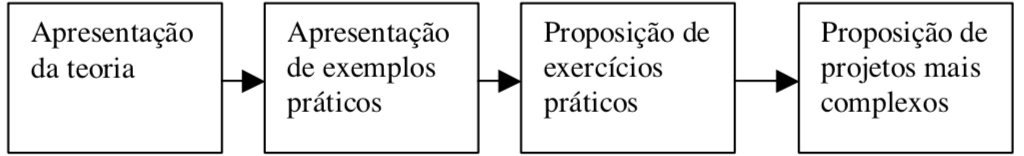
\includegraphics[keepaspectratio=true,scale=0.34]{figuras/modoTradicional.png}
	\caption{Sequência de passos típicos na apresentação de uma disciplina, \citeonline{Borges}}
	\label{figura4}
\end{figure}

Ao se apresentar uma nova liguagem de programação, é comum as aulas serem realizadas em laboratórios com
recursos computacionais. Apesar dessas aulas apresentarem um formato diferenciado em relação ao modo tradicional,
os professores não exploram a diversidade dos equipamentos disponíveis com práticas que apoiem o desenvolvimento 
de habilidades por parte dos estudantes \cite{Borges}.

\section{Gamificação}
Jogos são uma construção humana que envolvem em seu contexto fatores sociais, culturais e econômicos \cite{EaDF440}.
Como apresentado no livro "Gamificação na Educação" por \citeonline{da2014gamificaccao}, a interação com \textit{games}, apesar
dos custos altos dos consoles, foram ocupando cada vez mais o tempo das pessoas que notaram que os jogos poderiam ser boas fontes
de prazer e entretenimento.

O notável crescimento do mercado dos \textit{games} tem atraido diferentes olhares de estudiosos que se dedicam ao estudo de seu
uso na educação, comunicação, marketing, psicologia, computação, entre outras áreas \cite{da2014gamificaccao}.

O termo gamificação, segundo \citeonline{da2014gamificaccao}, consiste na utilização de elementos de jogos em 
atividades que por natureza de sua criação não são jogos. \citeonline{raposo2016desafio} dizem que o objetivo da gamificação, consiste em resolver
problemas práticos ou despertar interesse e engajar um público específico para a realização de uma determinada
atividade. 

\subsection{Gamificação na Educação}
Embora o termo gamificação tenha sido apresentado pela primeira vez em 2010, a idéia de se utilizar
elementos de jogos em atividades que não são jogos, tem sido utilizado há muito tempo. Na educação
de crianças, por exemplo, as mesmas podiam ter seus esforços e trabalhos reconhecidos por meio
de estrelinhas ou outros tipos de recompensas dadas por seus educadores, como explica \citeonline{da2014gamificaccao}.

De acordo com \citeonline{da2014gamificaccao}, no Brasil existem diversas instituições públicas e privadas que apoiam o desenvolvimento e uso de ambientes
gamificados. A exemplo disto, o Ministério da Educação visa fornecer suporte para o ambiente gamificado de apoio ao ensino \textit{Geekie games} que possibilita
aos estudantes se prepararem para o Exame Nacional de Ensino Médio (ENEM). Os resultados da utilização da ferramenta, segundo \citeonline{da2014gamificaccao}, 
foram considerados positivos e o Ministério da Educação levanta a possibilidade de extender o uso da ferramenta gamificada para outros sistemas de avaliação.

Segundo \citeonline{hammer}, somente a utilização de elementos de jogos no ensino não resolve a falta de empatia no processoe de aprendizagem dos alunos
uma vez que a utilização de mecanismos como por exemplo o sistema de pontuação já estão presentes no cotidiano escolar há anos. De acordo com as autoras, 
a utilização de elementos e característica de jogos devem provocar impactos tanto emocionais quanto sociais nos indivíduos para que eles tenham um aprendizado
efetivo. 

\section{\textit{Framework Octalysis}}
No livro \textit{"Actionable Gamification – Beyond Points, Badges, and Leaderboards"}, \citeonline{chou2017actionable} apresenta uma série
de características que, segundo ele, atraem e motivam pessoas a tomarem decisões e a realizarem determinadas atividades.
\citeonline{chou2017actionable} ressalta ainda que essas características estão presentes na maioria dos jogos bem sucedidos.

Ao estudar uma variedade de técnicas de jogos que fazem com que os mesmos sejam tão atraentes, \citeonline{chou2017actionable} notou que estas 
técnicas impulsionam os jogadores de maneiras diferentes. Algumas estimulam os jogadores a permanecerem no jogo por meio da
inspiração e capacitação, outras estimulam por meio da manipulaçãoe e obsessão.

Com o aprofundamento de sua pesquisa e a partir da observação de como as técnicas de jogos influenciam nos jogadores, \citeonline{chou2017actionable} 
propôs uma estrutura de design de gamificação que foi apelidada de  \textit{Framework Octalysis}.

O \textit{Framework Octalysis} une elementos de \textit{design} de jogos com a psicologia objetivando motivar os envolvidos
no processo de gamificação a realizarem determinadas ações. O modelo de \citeonline{chou2017actionable} apresenta oito eixos principais que 
são chamados de \textit{core drives}, cada \textit{core} apresenta características que por sua vez apresentam técnicas que
influenciam diretamente os jogadores. Nas subseções a seguir, é apresentado cada um dos oito \textit{core drives}
definidos por Yu-Kai Chou.

\subsection{Significado épico e chamado}
Significado épico e chamado, segundo \citeonline{chou2017actionable}, é um \textit{core} que provoca a sensação no jogador de que ele está envolvido em algo 
grande e que foi especialmente escolhido para executar uma determinada ação. Ao realizar uma contribuição para a plataforma Wikipedia, por exemplo,
as pessoas acreditam que estão ajudando a proteger e disseminar algo que é maior que elas, o conhecimento humano \cite{chou2017actionable}. O próprio autor relata 
em seu livro a experiência que teve com a criação de uma página na Wikipedia com informações de sua empresa, página criada por ele permaneceu no ar por pouco minutos.
Vários contribuintes da Wikipedia relataram que a página não era significante o suficiente para merecer estar na Wikipedia, vários membros concordaram com
a insignificância da página e, após aproximadamente dez minuto a página foi retirada do ar. Para \citeonline{chou2017actionable}, isso 
ocorreu devido ao fato de as pessoas que constituiam a "comunidade Wikipedia", ao realizarem o trabalho voluntário de inspecionar os conteúdos da plataforma, sentirem
que estão fazendo parte de algo que é maior que elas e que de certa forma estão protegendo o conhecimento humano.

Abaixo são apresentadas duas das seis técnicas de "Significado épico e chamado" segundo \citeonline{chou2017actionable}.
As demais técnicas podem ser apreciadas em seu livro presentes no livro \textit{"Actionable Gamification – Beyond Points, Badges, and Leaderboards"}.

\begin{itemize}
	\item Narrativa: A maioria dos jogos iniciam com uma história que mostra aos jogadores o contexto sobre o qual está
	inserido o jogo e o quão importante o jogador é para solucionar os desafios propostos. Uma das maneiras mais eficazes
	em utilizar este núcleo é por meio de uma narrativa envolvente. 
	\item Herói da humanidade: Em seu livro, \citeonline{chou2017actionable} apresenta exemplos que demonstram a natureza desta
	técnica. A empresa \textit{"Tom's Shoes"}, por exemplo, envia um par de sapatos para uma criança em país de terceiro mundo sempre
	que um de seus clientes realiza um novo pedido. O site \textit{"Free Rice"} doa dez grãos de arroz para cada resposta correta dadas
	para as perguntas educacionais postadas no site. Mecanismos como este, passam a sensação de "heroismo" aos envolvidos, fazendo com que 
	os mesmos se sintam motivados em participar das atividades propostas.  

\end{itemize}

\subsection{Desenvolvimento e Conquista}
Desenvolvimento e conquista é o segundo \textit{core} do \textit{framework} e está relacionado à motivação interna de 
cada pessoa em desenvolver suas habilidades e superar desafios. Neste núclo, o desafio para se conquistar, por exemplo, 
um troféu ou distintivo é muito importante, uma vez que conquistar estes artefatos sem um desafio se torna insignificante.
De acordo com \citeonline{chou2017actionable}, essa é a unidade mais fácil de ser projetada. Alguns exemplos de artefatos utilizados
neste \textit{core}: pontuação, emblemas, \textit{ranking} e etc.

\subsection{Empoderamento e feedback}
Empoderamento e feedback é o terceiro \textit{core} e está ligado ao uso de táticas visando promover a realização pessoal
do usuário de forma a aumentar seu potencial. Geralmente é expresso quando os usuários se envolvem em um processo criativo
onde os mesmos descobrem coisas novas e, a partir disso, passam a tentar combinações novas, recebendo \textit{feedbacks}
de acordo com os resultados destas novas combinações.

\subsection{Propriedade e posse}
Propriedade e posse é o quarto \textit{core}. É onde os usuários são motivados a permanecerem nas atividades por
sentirem que possuem controle sobre aluguma coisa. De acordo com \citeonline{chou2017actionable}, quando uma pessoa
sente que tem propriedade sobre alguma coisa, a atitude dela é de querer aumentar e melhorar o que possui. Se uma pessoa
gasta muito tempo personalizando seu avatar, automaticamente sente mais propriedade e controle sobre ele ou quando ela é
recompensada com uma moeda virtual ou bens virtuais, a postura dela é realizar mais atividades objetivando receber
e acumular mais bens.

\subsection{Influência e relacionamento social}
Influência e relacionamento social é o quinto \textit{core} e envolve todos os elementos e características sociais que 
motivam as pessoas. São alguns destes elementos: aceitação social, competição, feedback social e até inveja. Em seu livro,
\citeonline{chou2017actionable} diz que, quando vemos um amigo que possui uma ótima habilidade em alguma coisa, logo nos sentimos
motivados a alcançar o mesmo. Quando alguém nos fala que um determinado nível em um jogo, por exemplo, a nossa reação, na maioria das 
vezes, é de querer superar a pessoa e, portanto nos engajamos para realizar tal feito.

\subsection{Escassez e impaciência}
A escassez e a impaciência é o sexto \textit{core} e consiste na urgência de se obter algo só porque é raro, exclusivo ou inatingível. De 
acordo com \citeonline{chou2017actionable}, o facebook, por exemplo, na época em que foi lançado era exclusivo para estudantes de \textit{Harvard}, 
depois foi aberto para outras Universidades de grande prestígio e finalmente, quando aberta para todos os público, universitários ou não, 
houve um grande aumento no número de pessoas que queriam participar da rede social pelo simples fato de que anteriormente não podiam.

\subsection{Imprevisibilidade e curiosidade}
Imprevisibilidade e curiosidade é o sétimo \textit{core} e exige o envolvimento constante, uma vez que não se tem nenhuma previsão
do que acontecerá. \citeonline{chou2017actionable} explica que, quando algo não se enquadra nos nossos ciclos regulares de reconhecimento
de padrões, nosso cérebro entra em ação e passa a focar no inesperado, predendo nossa atenção ao que pode vir a ocorrer. Yu-Kai Chou explica
ainda que esse é o principal núcleo por trás dos vícios dos jogos de azar.

\subsection{Prevenção e perda}
Prevenção e perda é o oitavo e último \textit{core} do \textit{framework} e está relacionado à motivação em se evitar que algo negativo
aconteça. Exemplo: realizar alguma ação em um jogo para evitar que pontos sejam perdidos por falta de atividade.

\section{Elementos motivacionais: Octógono}
De acordo com \citeonline{chou2017actionable}, tudo o que se faz em relação à gamificação é baseado em um ou mais \textit{core drives}. 
Quando não há nenhum dos oito núcleos, a motivação é zero e nenhuma atividade é realizada.

\subsection{Divisão dos motivadores de acordo com sua natureza}

Cada um dos oito \textit{core drives} possuem naturezas diferentes. Alguns fazem os usuários se sentirem poderosos mas não criam a 
sensação de urgência, outros já criam essa sensação nos usuários, além de obsessão e vício. Como resultado destas diferentes características,
as oito unidades do \textit{framework} são mapeadas em um octógono onde a posição de cada um determina a natureza da motivação. Na figura \ref{octogono}
é apresentado a distribuição de cada \textit{core drive} no octógono.

\begin{figure}[h]
	\centering
	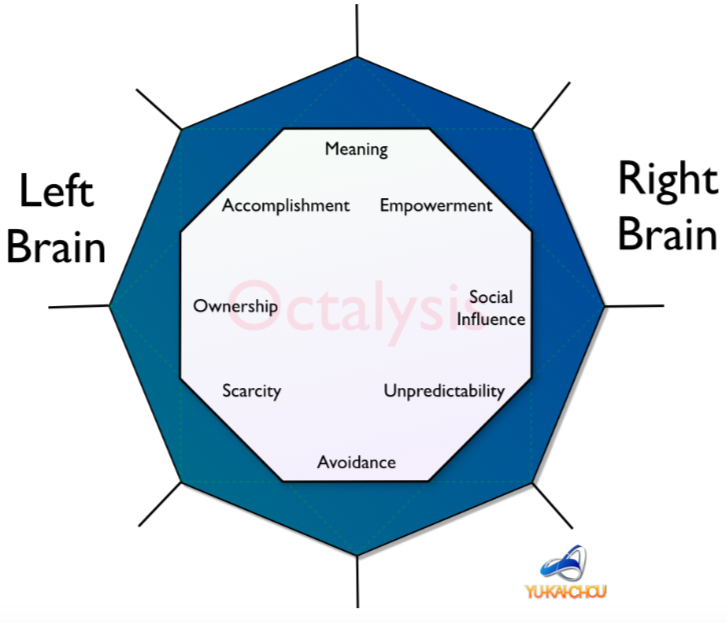
\includegraphics[keepaspectratio=true,scale=0.34]{figuras/brain.png}
	\caption{Divisão do octógono, \citeonline{chou2017actionable}}
	\label{octogono}
\end{figure}

A estrutura de \textit{Octalysis} é organizada de forma que os núcleos relacionados à criatividade, auto expressão e dinâmica social são
representados dos lado direito do octógono ("\textit{Right Brain}"). Os núcleos relacionados à logica, pensamento analítico e propriedade são representados graficamente
no lado esquerdo (\textit{"Left Brain"}). É importante ressaltar que "\textit{Right Brain}" e \textit{"Left Brain"} não são literais no que se refere
à regiões do cérebro humano, a utilização destes termos é apenas um simbolismo.

\subsection{Gamificação \textit{White Hat} e \textit{Black Hat}}

Uma característica importante na representação dos núcleos motivacionais dentro do octógono é a forma como eles estão agrupados em relação ao impacto
que causam sobre os participantes. Os núcleos localizados na parte superior do octógono são considerados "motivadores positivos" enquanto os núcleos localizados
na parte inferior do octógono são considerados "motivadores negativos". Os \textit{cores} apresentados na parte superior são chamados de \textit{"White hat"} e os inferiores
são conhecidos como \textit{"Black hat}. Na figura \ref{octogono} é apresentado a divisão dos núcleos levando em consideração o tipo de motivador em que cada um
é classificado.

\begin{figure}[h]
	\centering
	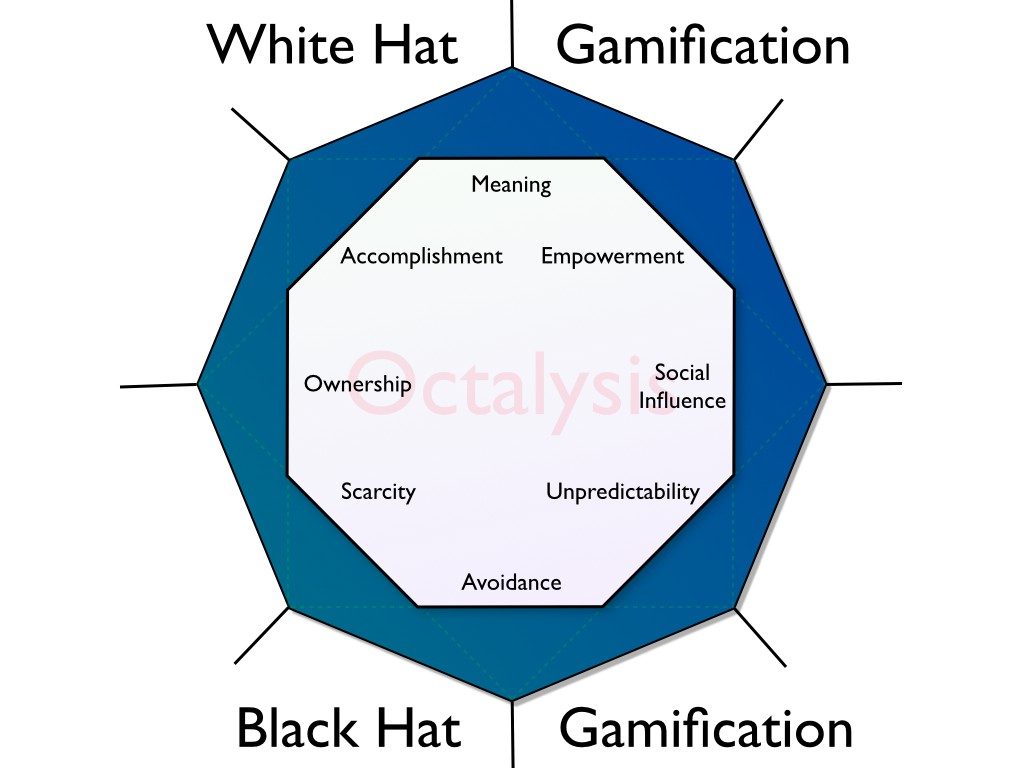
\includegraphics[keepaspectratio=true,scale=0.28]{figuras/octogono.jpg}
	\caption{Gamificação \textit{White hat} e \textit{Black hat}, \citeonline{chou2017actionable}}
	\label{octogono}
\end{figure}

\citeonline{chou2017actionable} apresenta um exemplo do que vem a ser os núcleos \textit{"White hat"} e \textit{"Black hat"}. Se algo é envolvente
por permitir que se expresse a criatividade, faz com que os indivíduos envolvidos se sintam bem sucedidos e poderosos, com certeza há um \textit{core} 
\textit{"White hat"} sendo utilizado. Por outro lado, se os envolvidos realizam determinadas ações por não saber o que acontecerá logo em seguida ou está
constantemente com medo que algo ruim possa acontecer, neste caso, há um \textit{core} \textit{"Black hat"} sendo utilizado.

Como apresentado por \citeonline{chou2017actionable}, não é porque alguma coisa é categorizada como \textit{"black"} que ela seja ruim. Se utilizadas
corretamente podem gerar resultados saudáveis e positivos. De acordo com \citeonline{chou2017actionable}, um profissional de gamificação deve sempre considerar
todos os \textit{core drive} objetivando obter resultados positivos e produtivos.


\section{Estudos semelhantes}
% Com o objetivo de apoiar o ensino e aprendizagem de programação, alguns autores investem no estudo e desenvolvimento
% de ferramentas que possam aumentar o interesse e engajamento de alunos na realização de determinadas atividade. Nesta
% seção, são apresentadas algumas tecnologias, segundo a literatura, que foram desenvolvidas com o objetivo de auxiliar
% alunos e professores no ensino e aprendizagem de programação.

% \section{Exemplo de Ferramenta gamificada existente}
Com o objetivo de apoiar o ensino e aprendizagem de programação, alguns autores investem no estudo e desenvolvimento
de ferramentas que possam aumentar o interesse e engajamento de alunos na realização de determinadas atividades. Nesta
seção, é apresentada uma tecnologia desenvolvida por pesquisadores da Universidade Federal da Paraíba com o objetivo de auxiliar
alunos e professores no ensino e aprendizagem de programação.

\subsection{O Desafio da Serpente}
Tendo em vista os problemas motivacionais e dificuldades enfrentadas por alunos de graduação no que se refere ao
aprendizado de programação do curso de computação da Universidade Federal
da Paraíba, \citeonline{raposo2016desafio} desenvolveram um jogo que foi disponibilizado na \textit{web} {\itshape} e apelidado
de "O Desafio da Serpente". O propósito da criação do jogo é estimular os alunos a praticarem diariamente seus conhecimentos
por meio de uma série de questões selecionadas e disponibilizadas pelo professor da disciplina.

O jogo envolve os alunos em uma batalha contra uma serpente que faz referência à linguagem de programação utilizada na
disciplina (\textit{python}{\itshape}). Para enfrentar e derrotar a serpente, os jogadores devem conquistar armas mediante o acúmulo
de pontos e resolução dos desafios propostos. 

Em seguida é apresentado um tabuleiro conceitual do jogo. No tabuleiro é possível
identificar por meio das diferentes cores as cinco fases propostas e as armas que podem ser conquistasdas mediante a
resolução dos desafios. O uso do corpo da serpente como tabuleiro tem como objetivo apresentar o caminho sequencial que deve
ser seguido pelos jogadores em busca da vitória. Cada fase, representadas pelas cores na figura \ref{figura1}, correspondem a um conteúdo
que deve ser estudado pelos jogadores.

\begin{figure}[h]
	\centering
	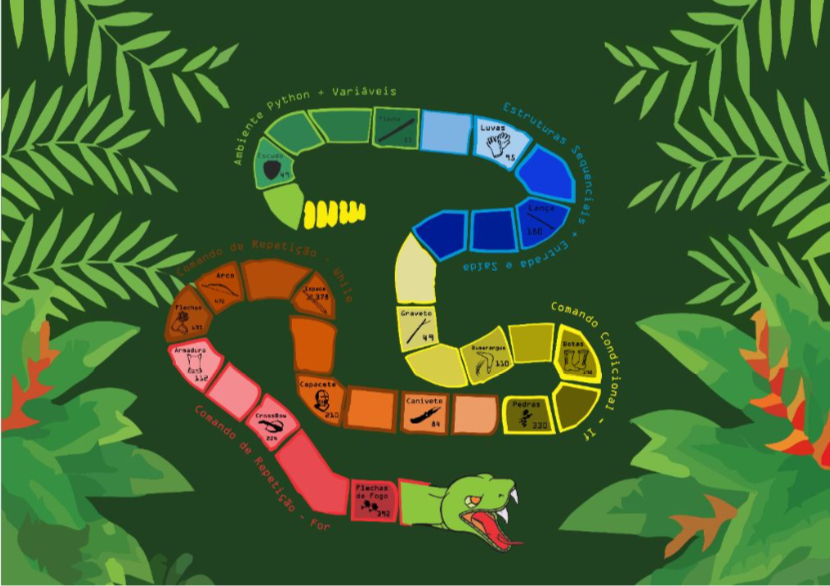
\includegraphics[keepaspectratio=true,scale=0.35]{figuras/desafioSerpente.png}
	\caption{Representação conceitual do jogo, \citeonline{raposo2016desafio}}
	\label{figura1}
\end{figure}

Todos os dias da semana, de segunda a sexta feira, eram disponibilizados desafios que continham de duas a seis
questões dos mais variados níveis de complexidade, permitindo que os jogadores, ao concluírem os desafios propostos, 
conquistassem pontos e adquirissem armas. O objetivo era estimular os jogadores a estabelecerem uma rotina de estudos,
dedicando diariamente algum tempo para a resolução de exercícios voltados para a programação.

As questões foram classificadas em três níveis de complexidade (fácil, médio e difícil), no quadro a seguir, apresenta-se
as características de cada um destes níveis.

\begin{table}[h]
	\centering
	\resizebox{\textwidth}{!}{%
	\begin{tabular}{|l|l|l|l|}
	\hline
	\textbf{Complexidade} & \textbf{Tipo de Questão} & \textbf{Tempos estimado para resposta} & \textbf{Quantidade máxima de questões por dia} \\ \hline
	Fácil & \begin{tabular}[c]{@{}l@{}}V ou F\\ Teórica Objetiva\end{tabular} & 5 minutos & 8 \\ \hline
	Médio & \begin{tabular}[c]{@{}l@{}}Acompanhamento\\  (Teste de Mesa)\end{tabular} & 10 minutos & 4 \\ \hline
	Difícil & \begin{tabular}[c]{@{}l@{}}Elaboração de\\ Programas\end{tabular} & 20 minutos & 2 \\ \hline
	\end{tabular}%
	}
	\caption{Classificação das questões, \citeonline{raposo2016desafio}}
	% \small{Quadro 1 - Classificação das questões, \citeonline{raposo2016desafio}} 
\end{table}

\pagebreak
Objetivando manter os jogadores motivados, cada fase possuia um sistema de (\textit{ranking}{\itshape}) independente
das fases anteriores, desta forma, mesmo que um jogador não tivesse obtido uma boa pontuação nas fases anteriores, ele
começaria a fase seguinte sem desvantagem em relação aos demais jogadores. 

A medida que os jogadores acumulavam pontos, os mesmos conquistavam novas armas para combater a serpente. Estas armas podiam
ser de defesa (escudos,armaduras e etc) ou de ataque (espada, lança e etc). O objetivo era fazer com que os jogadores conseguissem conquistar
o maior número possível de armas em cada fase. Cada armamento possuia uma quantidade mínima de pontos necessários para sua
aquisição e possuiam apenas funções simbólicas..

\begin{figure}[h]
	\centering
	
\includegraphics[keepaspectratio=true,scale=0.45]{figuras/armas.png}
	\caption{Exemplos de armas e pontuações, \citeonline{raposo2016desafio}}
	\label{figura2}
\end{figure}

Além de permitir que os jogadores colecionassem pontos e armas, os primeiros jogadores tinham sua fotos expostas no
site do jogo, exaltando suas conquistas.

Para motivar os alunos a utilizarem a ferramenta e possibilitar a coleta de dados que permitissem analisar o 
impacto do uso da tecnologia gamificada no ensino de programação, foi acordado que, os alunos que obtivessem 
um aproveitamento de no mínimo 70\% em todas as fases do jogo, receberiam um ponto extra na primeira unidade 
da disciplina. Os alunos que obtivessem nota superior ou igual a 50\% em todas as fases do jogo, receberiam 
meio ponto extra na nota da primeira unidade da disciplina. Desta forma, a participação no jogo teria caráter 
voluntário e não estaria diretamente ligado às avaliações da disciplina. Recompensar os alunos com pontos extras
tinha como objetivo identificar até que ponto a motivação dos jogadores em solucionar os desafios seria ocasionado
pelo próprio jogo e não por pontos.

Considerando as quatro primeiras semanas de aula utilizando a ferramenta, os resultados foram bastante animadores.
Do total de 106 alunos que realmente frequentaram as aulas, apenas quatro não participaram de nenhum dos desafios 
propostos, o que indica que a aceitação da ferramenta pelos alunos foi de mais de 96\% . Além destes indicadores 
quantitativos, \cite{raposo2016desafio} relatou em sua pesquisa que a empolgação dos alunos na utilização da 
ferramenta era bastante perceptível. Muitos alunos se diziam bastante ansiosos para o desafio do dia e notou-se um 
grande aumento no número de discussões a respeito das questões durante as aulas.

\chapter{Metodologia}

\section{Elicitação de requisitos}
Com o objetivo de levantar requisitos para a construção da ferramenta de apoio ao ensino e aprendizagem de 
programação, foi elaborado um questionário para coletar informações a respeito da disciplina introdutória de programação 
do campus Gama (FGA) da universidade de Brasília na visão dos alunos que cursaram ou estão cursando a disciplina. Também 
foram incluidas  questões relacionadas aos \textit{games} com o objetivo de identificar alguns mecanismos característicos
de jogos que pudessem ser incluidos na construção da ferramenta levando em consideração o  \textit{framework octalysis}
apresentado no capítulo 2 deste trabalho.

Ao se concluir a pesquisa baseada no questionário, iniciou-se a pesquisa por plataformas gamificadas semelhantes, buscando
identificar os mecanismos mais utilizados nestas ferramentas (sistema de \textit{ranking}, disputas e etc), usabilidade (layouts, responsividade e etc) entre outras.

Nas subseções a seguir, são apresentadas em detalhes a elaboração e resultados obtidos a partir das pesquisas realizadas.

\subsection{Questionário}
Para realizar a coleta de informações que permitissem a identificação dos requisitos, foi elaborado um questionário 
contendo XXX perguntas referentes à disciplina Algoritmos de Programação de Computadores e algumas outra perguntas
relacionadas à jogos na perspectiva do participante do questionário. Em seguida, o questionário foi publicado em um grupo na rede social \textit{facebook} que contém
vários estudantes dos cursos de engenharias da Universidade de Brasília (UnB), campus Gama (FGA). O mesmo questionário
também foi disponibilizado em um grupo no \textit{telegram} da engenharia de software criado pelos próprios estudantes do
curso. 

Disponibilizar o questionário no grupo do \textit{facebook} em que se encontram alunos de cada uma das cinco engenharias ofertadas no campus (FGA)
teve como objetivo reunir o maior número possível de informações sobre a perspectiva de diferentes perfis de alunos que cursam, cursaram ou vão
cursar a disciplina introdutória de programação.


As perguntas realizadas podem ser encontradas no anexo XXX deste trabalho.

% tabela com as perguntas aqui e percentual de respostas em uma das coluna
\subsection{Ferramentas Semelhantes}
Algumas ferramentas disponibilizadas na \textit{web} já apresentam características de jogos e , por conta disso,
atraem um grande público que utilizam destes recursos para aprimorar seus conhecimentos em programação, como é
o caso da plataforma \textit{Uri Online Judge} que é utilizada por cerca de 101.238 usuários atualmente e está disponível em três
idiomas, incluindo o português.
Nesta seção são apresentadas algumas das tecnologias gamificadas voltadas para o ensino e prática de programação
gamificadas. Algumas características de \textit{games} identificadas nestas ferramentas foram utilizadas como fonte
para o desenvolvimento da ferramenta proposta ao se notar sua grande utilização e aceitação após a comparação com as 
informações coletadas com o questionário.

\subsubsection{\textit{URI Online Judge}}
O URI Online Judge é uma ferramenta online disponível em três idiomas que permite que interessados em aprender ou
aprimorar seus conhecimentos em programação possam faze-lo de forma gamificada e intuitiva. A ferramenta possui três
formas de rankeamento que são: individual, por universidade ou por país. Até a data de publicação deste trabalho, o Brasil
lidera o \textit{ranking} de exercícios resolvidos e quantidade de usuários com 37.23.579 de exercícios resolvidos e cerca
de 101.238 usuários. \cite{URI} 

A ferramenta permite que seus usuários criem times e participem de torneios de duração que variam de trinta minutos até no 
máximo cinco dias, onde os jogadores batalham uns contra os outros na resolução de problemas relativos à programação.

O URI possui nove categorias de problemas que vão do nível mais básico (iniciante) até os mais complexos envolvendo grafos,
geometria computacional, linguagem sql entre outros.

Além da grande diversidade de categorias de problemas, a ferramenta permite que o usuário escolha a linguagem que deseja
praticar suas habilidades e conhecimentos em programação. No total são dezoito linguagens de programação que o jogador pode 
escolher.

\subsubsection{\textit{Data camp}}

% \subsection{Entrevistas}



\subsection{Priorização de requisitos: \textit{Moscow}}
Após concluir a coleta de informações, foi elaborado a tabela que é apresentada logo em seguida contendo os requisitos
identificados.

\begin{table}[h]
	\centering
	\resizebox{.8\textwidth}{!}{%
	\begin{tabular}{|l|l|l|l|}
	\hline
	\textbf{Identificador} & \textbf{Requisito}\\ \hline
	RF 01 & bla bla bla bla bla bla bla bla bla bla \\ \hline
	\end{tabular}%
	}
	\caption{Requisitos Funcionais}
	% \small{Quadro 2 - Requisitos funcionais} 
\end{table}

Com base na tabela apresentada anteriormente, utilizou-se a técnica de priorização de requisitos \textit{moscow} para realizar
a priorização dos requisitos. Esta técnica consiste na utilização de um quadro dividido em quatro colunas que servem como "classificadores"
de prioridade.\cite{moscow}

Logo em seguida são apresentados resumidamente cada um das quatro possíveis classificações abordadas pela técnica.
\begin{itemize}
	\item  \textit{Must Have}: nesta coluna vão todos os requisitos que críticos ou obrigatórios para a construção do sistema. Se um dos ítens
não é concluído, o projeto não é considerado bem sucedido;
	\item  \textit{Should Have}: itens com classificação \textit{should} são importantes mas não são necessários para entrega em um primeiro 
momento. São ítens tão importantes quanto os classificados como \textit{must}, mas em geral não são críticos ou pode-se esperar um pouco para ser
trabalhado;
	\item \textit{Could Have}: Ítens com esta classificação são desejáveis, mas não são necessários. Geralmente podem ser atendidos quando 
houver tempo e recursos disponíveis para sua realização.
	\item \textit{Would Have}: Ítens com esta classificação são os menos críticos ou não são adequados para serem realizados durante algum
período de tempo.
\end{itemize}

Segundo \citeonline{moscow}, algumas vantagens de se utilizar a técnica \textit{moscow} são: facilidade de compreensão, facilidade de trabalho, linguagem simples
entre outras. É importante salientar que se trata de uma técnica subjetiva quando se refere à classificação dos ítens e por este motivo, demanda de um 
bom entendimento do problema que se tem a intenção de resolver, de forma a melhor identificar quais ítens são de fato prioridades em relação à outros ítens.

Em seguida é apresentado um diagrama que torna o entendimento da utilização técnica \textit{moscow} mais simples.

\begin{figure}[h]
	\centering
	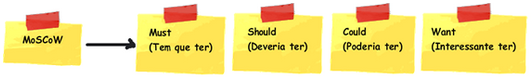
\includegraphics[keepaspectratio=true,scale=0.75]{figuras/moscow.png}
	\caption{Exemplificação da classificação de ítens quanto à sua prioridade, \cite{moscow}}
	\label{moscow}
\end{figure}

Na figura \ref{moscow} é apresentado uma esquematização simplificada quanto à utilização do \textit{moscow} como 
técnica de priorização de requisitos. É possível notar a redução gradativa da prioridade dos ítens quanto a sua necessidade
e urgência de desenvolvimento. 


\subsubsection{Escolha e implementação de \textit{core drives}}
Com base nas pesquisas realizadas que envolveu a aplicação de um questionário e observação de ferramentas semelhantas voltadas
para o ensino de programação como \textit{URI - Online judge} e \textit{Data camp} e, a partir da priorização dos requitos identificados
com as pesquisas....................


\subsection{Desenvolvimento: metodologia cascata}
De acordo com \citeonline{semedo2012ganhos}, metodologia pode ser definida como um conjunto de procedimentos, técnicas, documentação e ferramentas que 
auxiliam os responsáveis ou interessados no desenvolvimento e implementação de um sistema de informação. Na maioria das vezes, o sucesso
de um projeto de software depende de vários fatores que vão desde o planejamento à escolha mais adequada de uma metodologia.

O modelo cascata, também conhecido como modelo tradicional, é uma das metodologias mais antigas e conhecidas. A utilização desta 
metodologia consiste em seguir o desenvolvimento do projeto de forma sequencial, onde só se deve passar para os níveis seguintes após
a conclusão do nível anterior. Esta metodologia envolve duas grandes fases: levantamento de requisitos/necessidades e design. \cite{semedo2012ganhos}

Muitos autores desencorajam a utilização da metodologia cascata no desenvolvimento de grandes sistemas, como é o caso do pesquisador
\apudonline{gilb1988principles}{semedo2012ganhos}  e \apudonline{brooks}{semedo2012ganhos}. Este tipo de metodologia deve ser usada apenas em situações onde os requisitos do software são estáveis e requisitos
que possam vir a surgir no futuro sejam previsíveis. \cite{semedo2012ganhos}

\subsection{Arquitetura}

No desenvolvimento da ferramenta, tem-se como modelo arquitetural a ser utilizado o "n camadas". Esse tipo
de arquitetura consiste na separação de responsabilidades específicas para cada uma das camadas presentes 
na construção do sistema \cite{MSF}.

O modelo arquitetural simplificado, principais tecnologias e como essas tecnologias se comunicam pode ser observado 
na figura a seguir.

\begin{figure}[h]
	\centering
	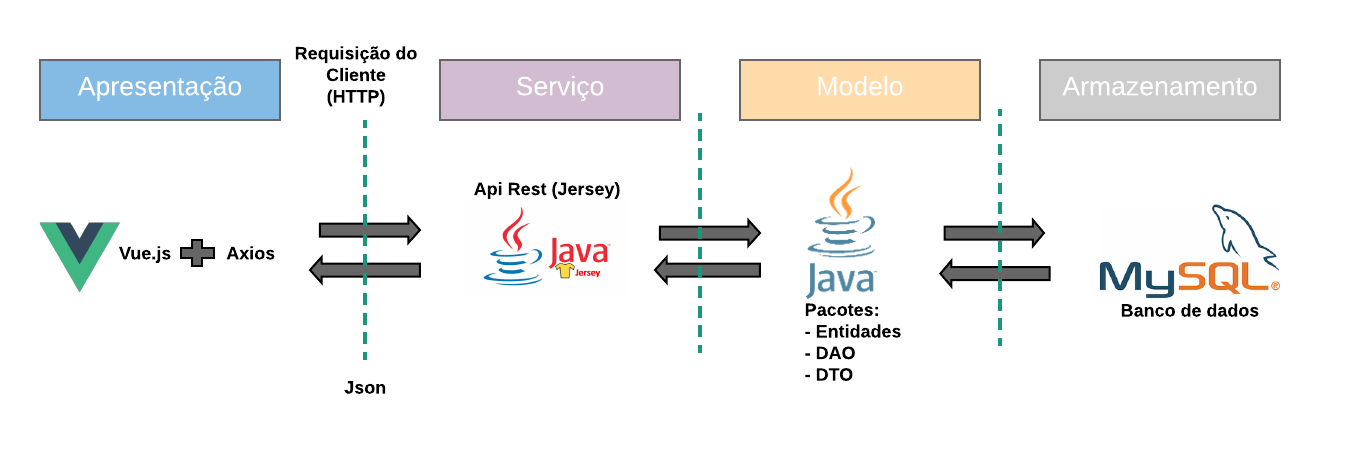
\includegraphics[keepaspectratio=true,scale=0.25]{figuras/arquitetura.png}
	\caption{Representação simplificada da arquitetura do sistema.}
	\label{arquitetura}
\end{figure}


\subsection{Tecnologias}

No desenvolvimento da ferramenta, escolheu-se as tecnologias com base nas seguintes características: afinidade
com as tecnologias de desenvolvimento, recursos disponibilizados pela tecnologia, qualidade e disponibilidade
de documentações e comunidades da tecnologia.

Nas subseções a seguir, são apresentadas resumidamente as principais tecnologias a serem utilizadas no desenvolvimento da 
ferramenta.

\subsubsection{Java}
\subsubsection{Vue.js}
\subsubsection{Mysql}
\subsubsection{Maven}
\subsubsection{Jersey}
Jersey

\begin{itemize}
	\item Levantamento de requisitos (questionários, literatura, ferramentas semelhantes, plano de ensino, currículo pedagógico e etc) -> tabelar
	\item Priorização de requisitos (usar o moscow?)
	\item Entrevistas (entrevistar colegas que já fizeram e estão fazendo)
	\item Conversas com professores
\end{itemize}

% (frameworks, bibliotecas e etc), documentação da tecnologia entre outros fatores que podem influenciar diretamente
% na construção do sistema.

% Para o desenvolvimento de uma solucão de software, deve-se considerar diversos
% fatores, como: afinidade com as tecnologias de auxílio ao desenvolvimento, recursos disponibilizados pela tecnologia 
% (frameworks, bibliotecas e etc), documentação da tecnologia entre outros fatores que podem influenciar diretamente
% na construção do sistema.

% No desenvolvimento desta ferramenta, a mesma foi dividida em duas áreas principais: backend e frontend. Para cada uma destas
% áreas, apresentamos a seguir as ferramentas utilizadas.


